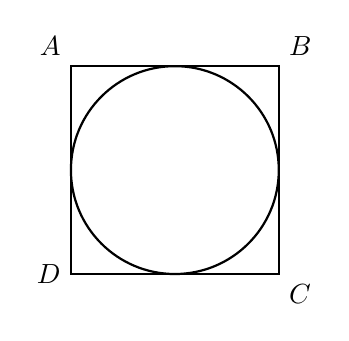
\begin{tikzpicture}[scale=0.6, thick]
	% Define the radius of the circle
	\def\r{2.2}
	
	% Draw the circle
	\draw (0,0) circle (\r cm);
	
	% Define vertices of the square circumscribing the circle
	\coordinate (A) at (-\r, \r);
	\coordinate (B) at (\r, \r);
	\coordinate (C) at (\r, -\r);
	\coordinate (D) at (-\r, -\r);
	
	% Draw the square
	\draw (A) -- (B) -- (C) -- (D) -- cycle;
	
	% Node labels for the vertices
	\node[above left] at (A) {$A$};
	\node[above right] at (B) {$B$};
	\node[below right] at (C) {$C$};
	\node[left] at (D) {$D$};
	
\end{tikzpicture}